\subsection{强化学习简介}

\begin{frame}{强化学习基础概念}

    \begin{columns}

        \column{0.55\textwidth}

        \begin{figure}
            \centering
            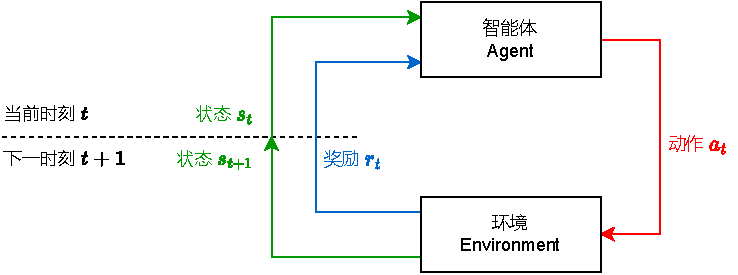
\includegraphics[scale=0.65]{pics/AgentInteractWithEnv.drawio.pdf}
            \caption{智能体与环境交互}
        \end{figure}

        \column{0.45\textwidth}

        \uncover<2->{
            我们将当前时刻 $t$ 及未来的奖励累加起来,记为回报 $u_t$ :
            \[u_t = r_t + r_{t+1} + r_{t+2} + r_{t+3} + \dots\]
        }

        \uncover<3->{
            为了使得回报 $u_t$ 能够收敛,我们引入折扣因子 $\gamma$ ,使得未来的奖励对当前的回报的贡献逐渐减小:
            \[u_t = r_t + \gamma r_{t+1} + \gamma^2 r_{t+2} + \gamma^3 r_{t+3} + \dots\]
        }

        \uncover<4->{
            我们的目标是最大化折扣回报 $u_t$ 。
        }

    \end{columns}

\end{frame}

\begin{frame}{以超级马里奥为例}

    \begin{figure}
        \centering
        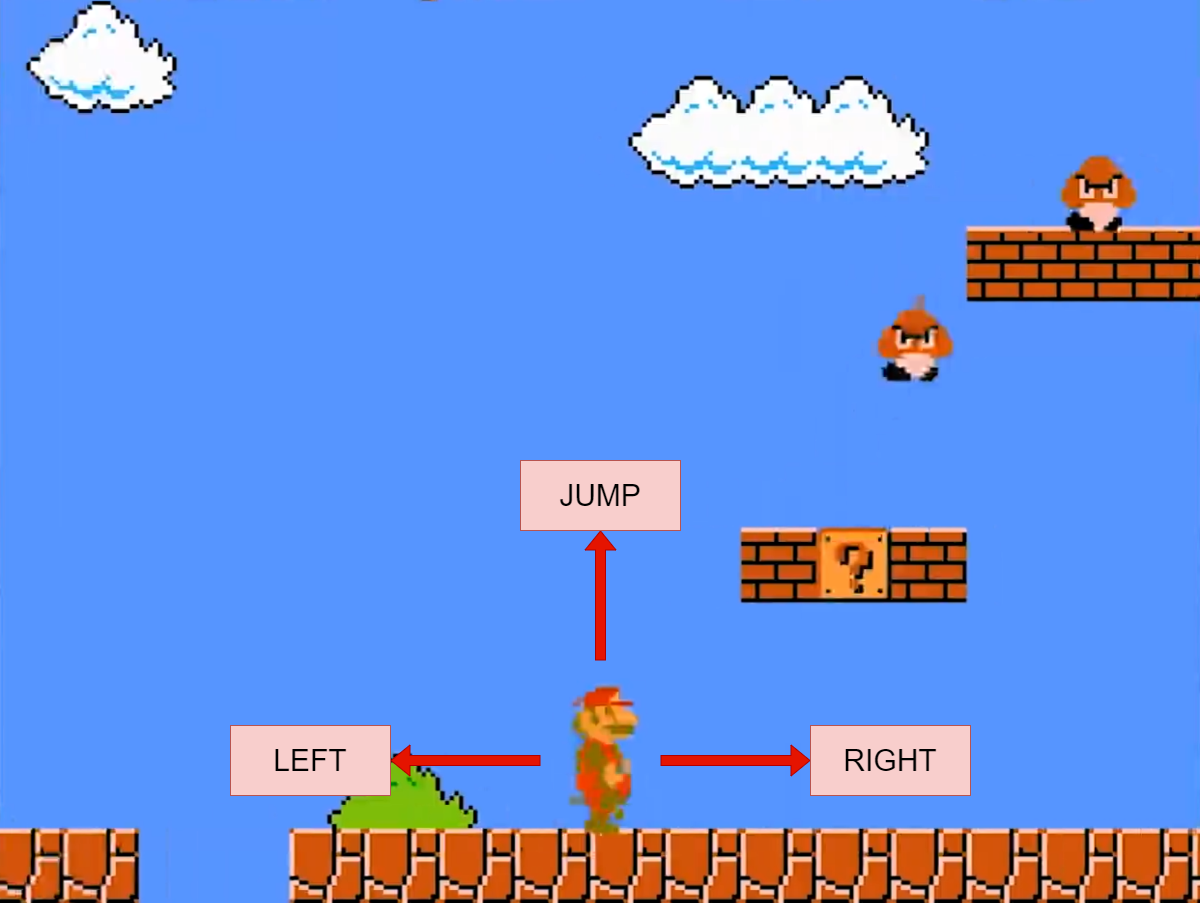
\includegraphics[scale=0.18]{pics/mario1.png}
        \caption{超级马里奥的动作空间}
    \end{figure}

\end{frame}

\begin{frame}{以超级马里奥为例}

    \begin{columns}

        \column{0.33\textwidth}

        \begin{figure}
            \centering
            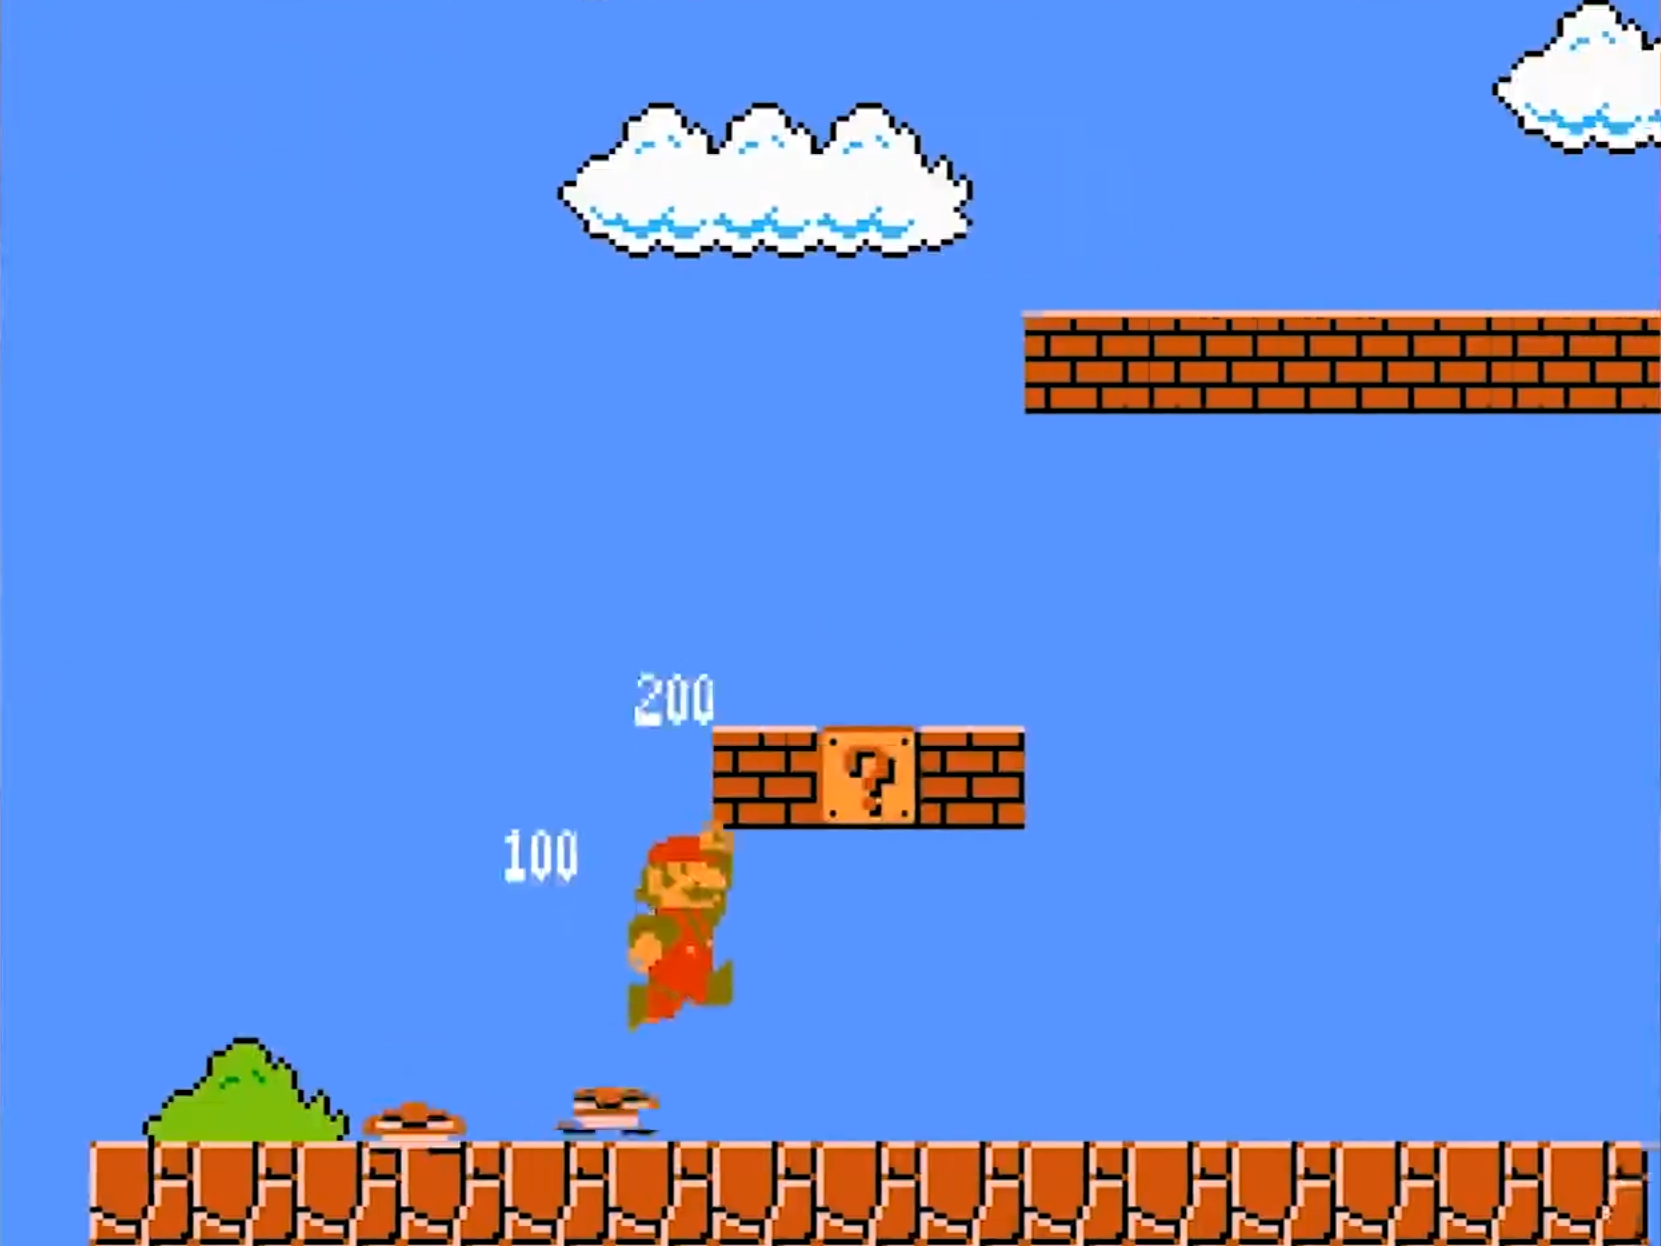
\includegraphics[scale=0.08]{pics/mario2.png}
            \caption{击杀怪物获得奖励}
        \end{figure}

        \column{0.33\textwidth}

        \begin{figure}
            \centering
            
\includegraphics[scale=0.08]{pics/mario3.png}
            \caption{收集金币获得奖励}
        \end{figure}

        \column{0.33\textwidth}

        \begin{figure}
            \centering
            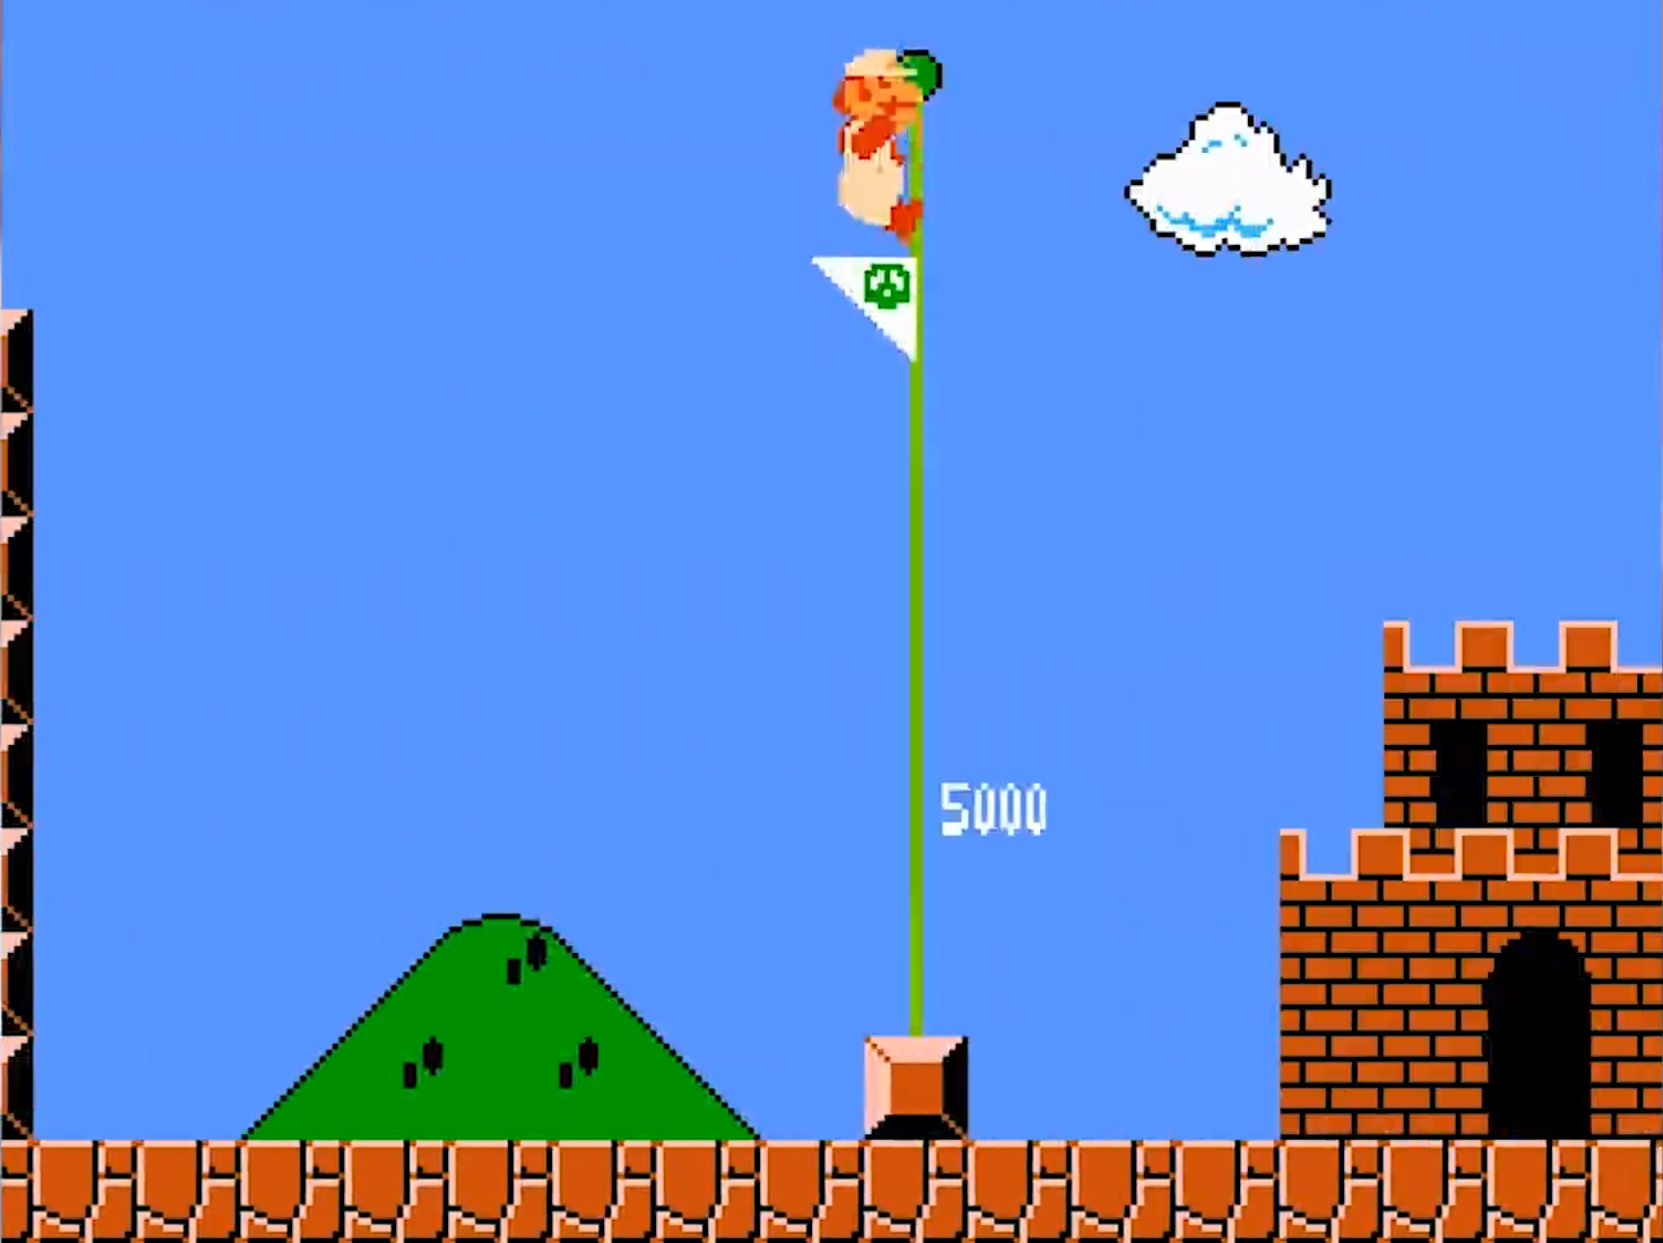
\includegraphics[scale=0.08]{pics/mario4.png}
            \caption{到达终点获得奖励}
        \end{figure}

    \end{columns}

\end{frame}

\begin{frame}{价值学习}

    由于状态、动作都具有随机性,所以通常将它们设为随机变量 $S$ 、$A$ 。
    又因为智能体获得的奖励取决于当前所处环境的状态以及执行的动作,所以累计折扣回报 $U_t$ 也是一个随机变量:
    \[U_t = R_t + \gamma R_{t+1} + \gamma^2 R_{t+2} + \gamma^3 R_{t+3} + \dots\]

    \uncover<2->{
    在 $t$ 时刻,我们只能得到当前环境的状态 $s_t$ 和智能体执行的动作 $a_t$ 。$t+1$ 时刻及之后的状态和动作都是未知的。
    因此我们对 $S_{t+1}, S_{t+2}, \dots$ 和 $A_{t+1}, A_{t+2}, \dots$ 求期望,以消除未知变量,记为 $Q$ :
    \[Q(s_t, a_t) = \mathbb{E}_{S_{t+1}, A_{t+1}, S_{t+2},  A_{t+2}, \dots}\left[U_t | S_t = s_t, A_t = a_t\right]\]
    其中 $Q(s_t, a_t)$ 称为\textcolor{blue}{动作价值函数}。它可以为状态 $s_t$ 下的动作 $a_t$ 打分,评分越高,动作越好。
    }

\end{frame}

\begin{frame}{价值学习}

    设 Agent 的动作空间 $\mathcal{A} = \{a_1, a_2, a_3\}$ ,$t$ 时刻观测到的状态 $S_t = s_t$ ,有:

    \begin{center}
        \begin{minipage}{0.7\textwidth}
            \begin{columns}
                \column{0.33\textwidth}
                $Q(s_t, a_1) = 20$
                \column{0.33\textwidth}
                $Q(s_t, a_2) = 100$
                \column{0.33\textwidth}
                $Q(s_t, a_3) = -50$
            \end{columns}
        \end{minipage}
    \end{center}

    Agent 应选择评分最高的动作执行,即 $a_t = a_2$ 。

    \uncover<2->{
        为了得到 $Q$ 函数,我们可以使用神经网络对其进行拟合:
        \begin{figure}
            \centering
            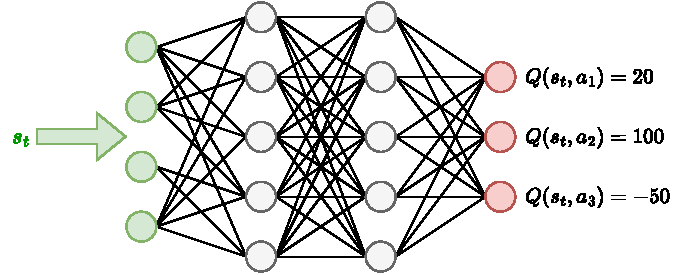
\includegraphics[scale=0.85]{pics/DQN.drawio.pdf}
            \caption{Deep Q-Network}
        \end{figure}
    }

\end{frame}

\subsection{云计算任务调度的场景模型}

\begin{frame}{云服务器任务调度模型}

    \begin{columns}
        \column{0.4\textwidth}

        任务调度流程:
        \begin{enumerate}
            \item 用户提交任务
            \item 任务进入任务队列
            \item 任务调度器使用\textcolor{blue}{调度算法},根据\textcolor{blue}{任务属性}和\textcolor{blue}{虚拟机状态}为任务分配虚拟机
        \end{enumerate}

        \column{0.6\textwidth}

        \begin{figure}
            \centering
            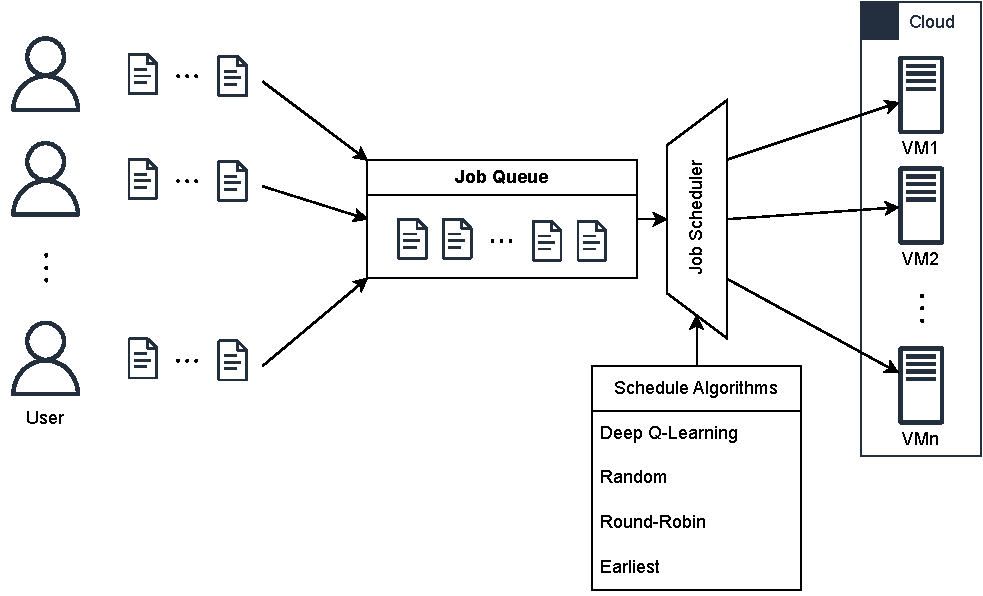
\includegraphics[width=\textwidth]{pics/module.drawio.pdf}
            \caption{云服务器任务调度模型}
        \end{figure}

    \end{columns}

\end{frame}
